\documentclass[a0paper,landscape]{baposter}

\usepackage{amsmath}
\usepackage{enumitem}
% Specify the theme for the poster
\usetheme{Simple}

% Metainfo
\author{Chenrui Wang, Yixuan Qiu}
\title{
    \parbox{\linewidth}{
        \centering
        The Sparse-Plus-Low-Rank Quasi-Newton Method \\ for Entropic-Regularized Optimal Transport
    }
}
\institute{
    Shanghai University of Finance and Economics
}

% Logo
% \titlegraphic{
%     
\includegraphics[height=8cm]{logos/ICML-logo.png}
%     \hspace{2cm}
%     
\includegraphics[height=8cm]{logos/SUFE_logo.png}
% }

\begin{document}

    \begin{poster}
    % poster settings
    {
        grid=false,
        columns=5,
        colspacing=0.7em,
        headerColorOne=cyan!20!white!90!black,
        borderColor=cyan!30!white!90!black,
        textborder=faded,
        headerborder=open,
        headershape=roundedright,
        headershade=plain,
        background=none,
        bgColorOne=cyan!10!white,
        headerheight=0.12\textheight
    }
    % Header
    {
        
\includegraphics[width=0.08\linewidth]{SUFE-logo.png}
    }
    % Title
    {\sc\huge\bf SPLR: The Sparse-Plus-Low-Rank Quasi-Newton Method for Entropic-Regularized Optimal Transport}
    % Authors
    {
        \vspace{0.3em}
        Chenrui Wang$^1$, Yixuan Qiu$^1$ \\[0.2em]
        $^1$ Shanghai University of Finance and Economics \\[0.2em]
    }
    % Conference Logo
    {
        \begin{tabular}{r}
            
\includegraphics[width=0.15\linewidth]{ICML-logo.png}
        \end{tabular}
    }

    \headerbox{\bf\color{sufered} Problem Definition}
{name=problem,column=0,row=0,span=1}
{
    Our goal is to solve the entropic-regularized optimal transport problem, and our approach is to study its dual problem. After removing one redundant degree of freedom, we obtain the \emph{smooth} and \emph{unconstrained} \emph{convex} optimization problem:
    \begin{align*}
    f(x)= & -\mathcal{L}(\alpha, \beta) \\
        = & \eta\sum\exp\{\eta^{-1}(\alpha_{i}+\beta_{j}-M_{ij})\}\nonumber\\
          & -\alpha^T a-\beta^T b, \label{eq:objective}
    \end{align*}
    where $x = (\alpha_1,\ldots,\alpha_n,\beta_1,\ldots,\beta_{m-1})^T$.
}
    \headerbox{\bf\color{sufered} Motivation}
{name=motivation,column=1,row=0,span=1}
{
    The main idea of SPLR is to provide an \emph{accurate approximation} of the Hessian matrix while maintaining its \emph{sparsity} as much as possible:
    \begin{itemize}
        \item \textbf{\color{sufered} Sparse:} Some second-order methods have been proposed based on the idea of Hessian sparsification. SPLR also obtain an approximation of the true Hessian matrix by sparsification.
        \item \textbf{\color{sufered} Low-Rank:} Similar to the BFGS update rule, we incorporate a low-rank correction term to enhance the approximation quality.
    \end{itemize}
}
    \headerbox{\bf\color{sufered} Contribution}
{name=contribution,column=0,span=2,below=problem}
{
    Our main contributions are summarized as follows:
    \begin{itemize}
        \item New theoretical results are developed to understand Hessian sparsification.
        \item A new quasi-Newton method is proposed to solve entropic-regularized OT with \emph{super-linear-like} convergence speed in practice.
        \item We provide convergence guarantees for the proposed method: SPLR enjoys a \emph{global convergence} property and the convergence speed is at least \emph{linear}.
        \item We conduct extensive numerical experiments to demonstrate the performance of SPLR on various entropic-regularized OT problems.
    \end{itemize}
}
    \headerbox{\bf\color{sufered} Hessian Sparsification}
{name=hessian-sparsification,column=0,below=contribution,span=2}
{
    Our sparsification scheme is designed based on the structure of the Hessian matrix, which preserves its diagonal elements and symmetry. The impact of this sparsification on the eigenvalues of the Hessian matrix is then analyzed under a \emph{very weak} assumption, leading to the following results:
    \begin{itemize}
        \item \emph{Any} valid sparsification scheme maintains positive definiteness.
        \item The sparsified Hessian matrix is guaranteed to have a smaller condition number. In particular, the biggest eigenvalue is reduced and the smallest eigenvalue is increased.
        \item The assumption is valid for almost \emph{any} sparsification scheme, allowing for highly flexible algorithmic designs and \emph{extremely sparse} matrices.
    \end{itemize}
    The assumption merely requires the existence of a power of the sparsified Hessian matrix in which all entries are strictly positive. A numerical verification is shown below:

    \vspace{0.5em}

    \begin{center}
    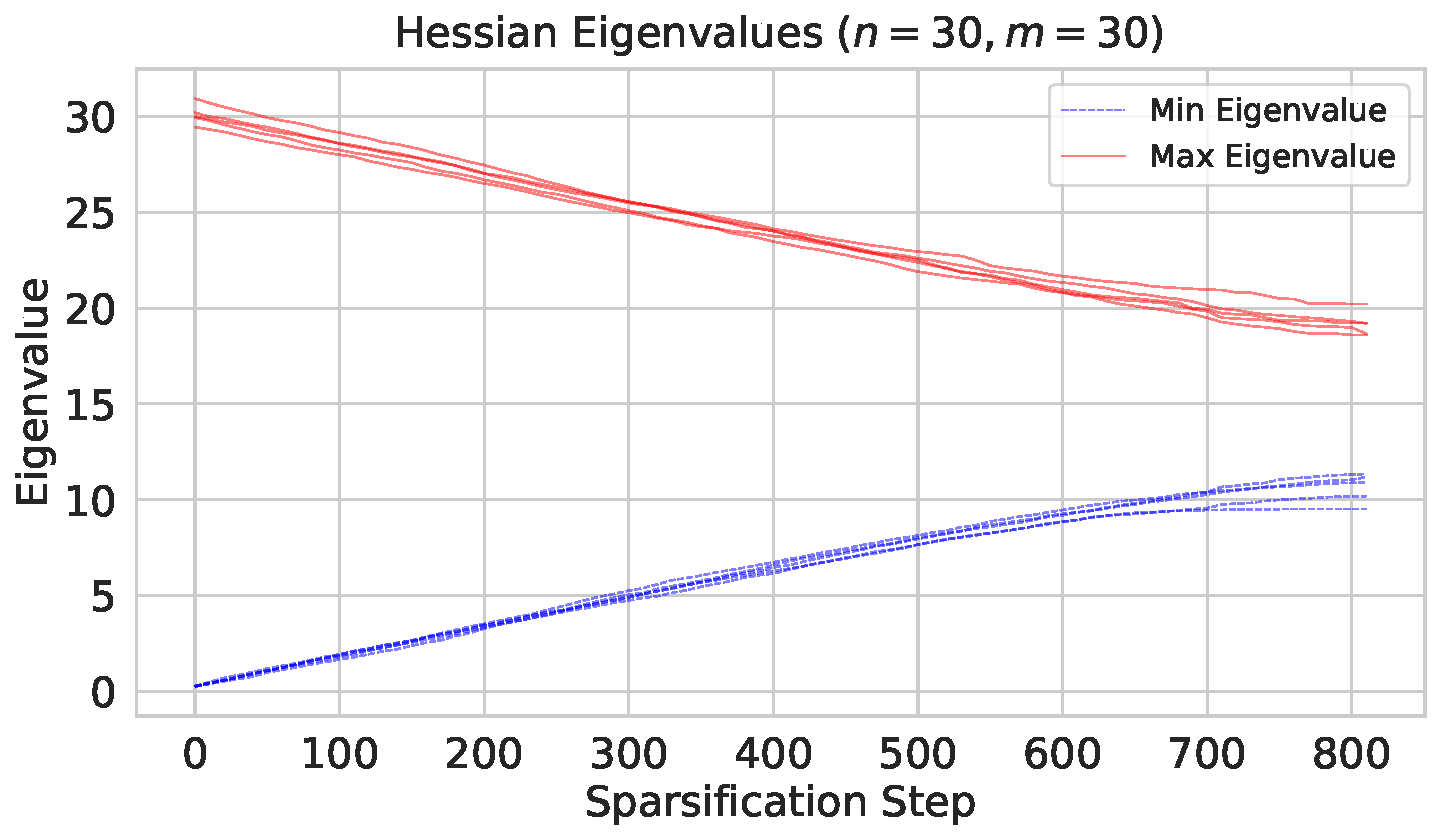
\includegraphics[width=0.48\textwidth]{save/eigen/eigenvalues_n30_m30.pdf}
    \hfill
    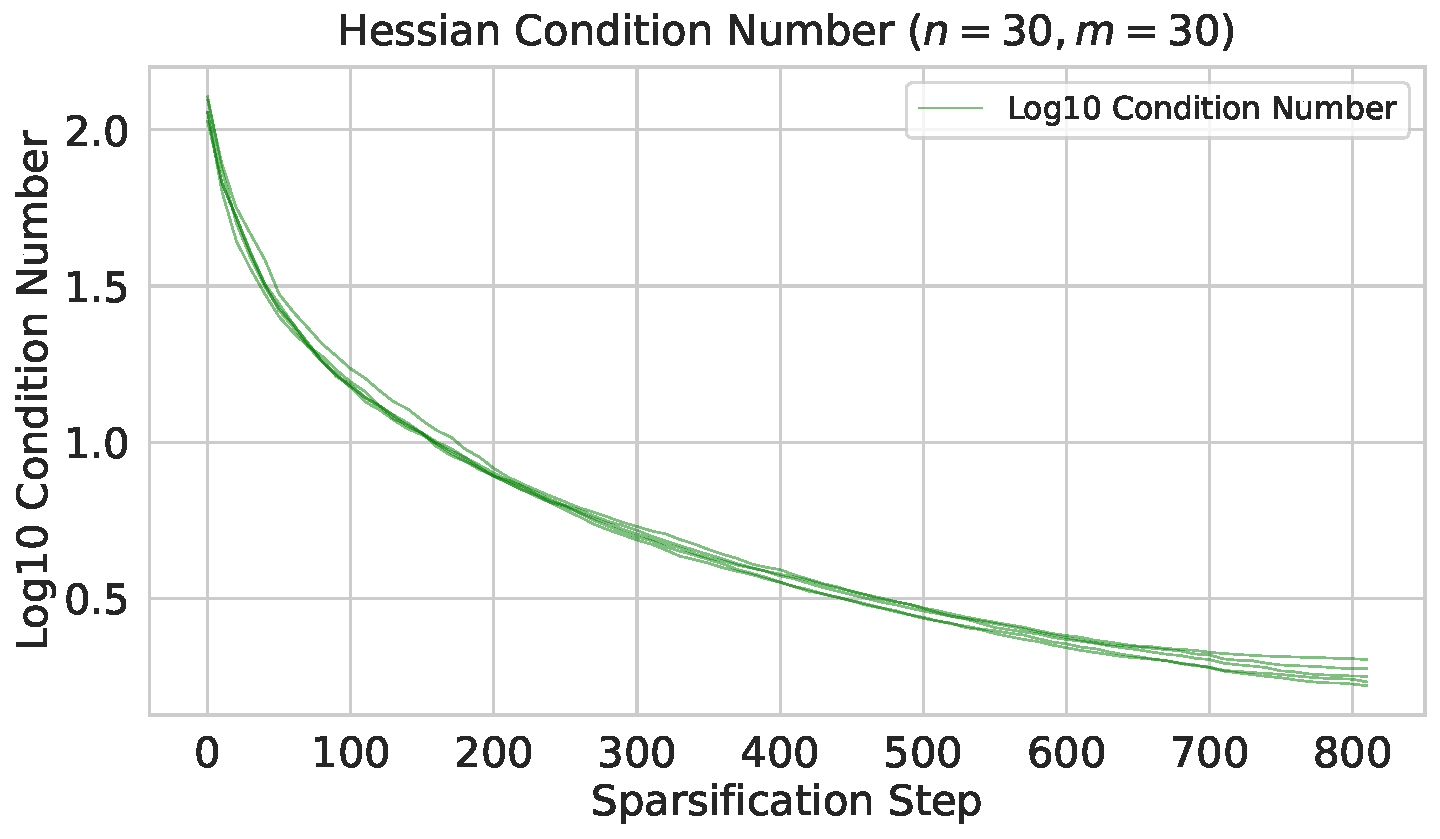
\includegraphics[width=0.48\textwidth]{save/eigen/condition_number_n30_m30.pdf}
    \end{center}
}

    \headerbox{\bf\color{sufered} Experiments}
{name=experiments,column=2,row=0,span=3}
{
    \begin{minipage}[t]{0.5\textwidth}
        \textbf{\color{sufered}Synthetic Datasets for Training:} 
        \vspace{-0.2em}
        \begin{center}
            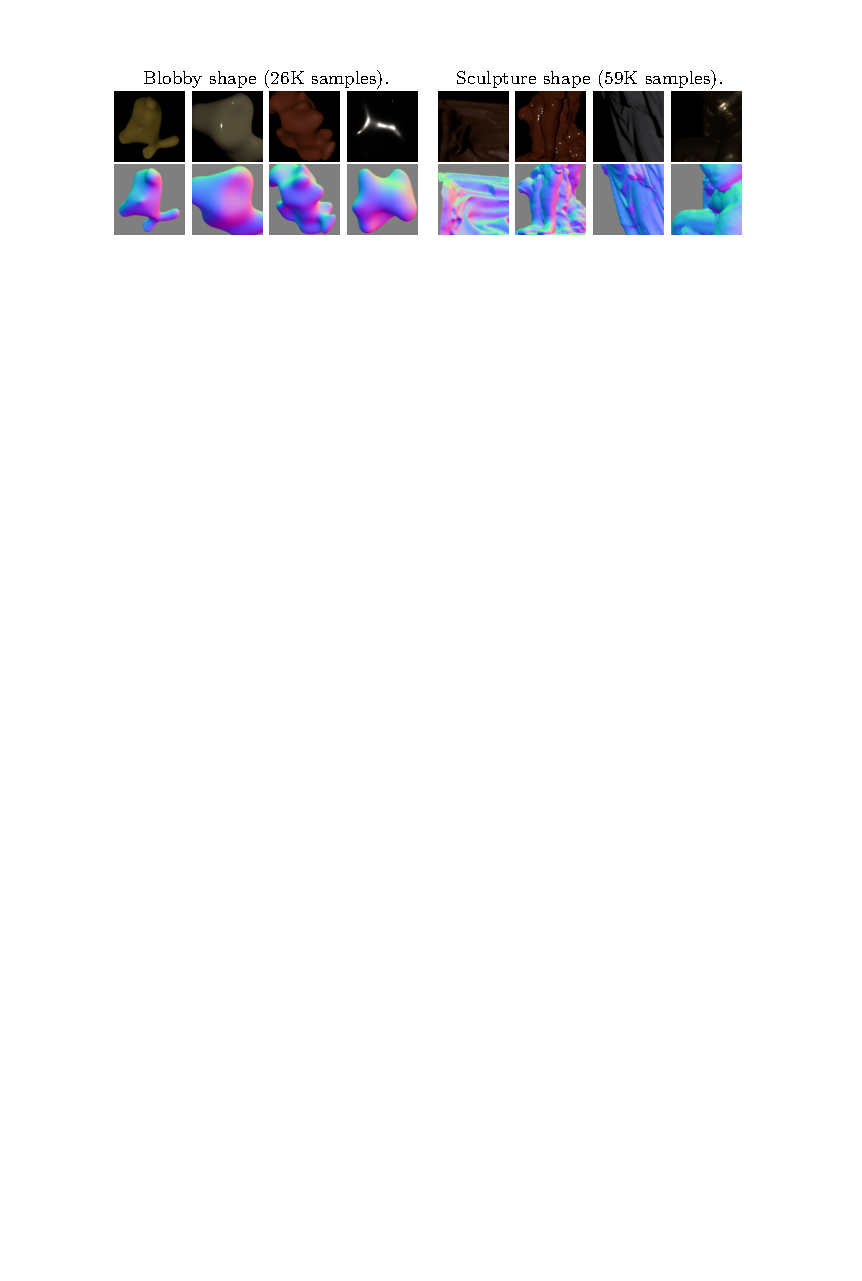
\includegraphics[width=\textwidth]{images/datasets.pdf}
        \end{center}
    \end{minipage}
    \begin{minipage}[t]{0.5\textwidth}
        \textbf{\color{sufered}Quantitative Results on DiLiGenT Main Dataset:} 
        \vspace{-0.2em}
        \begin{center}
            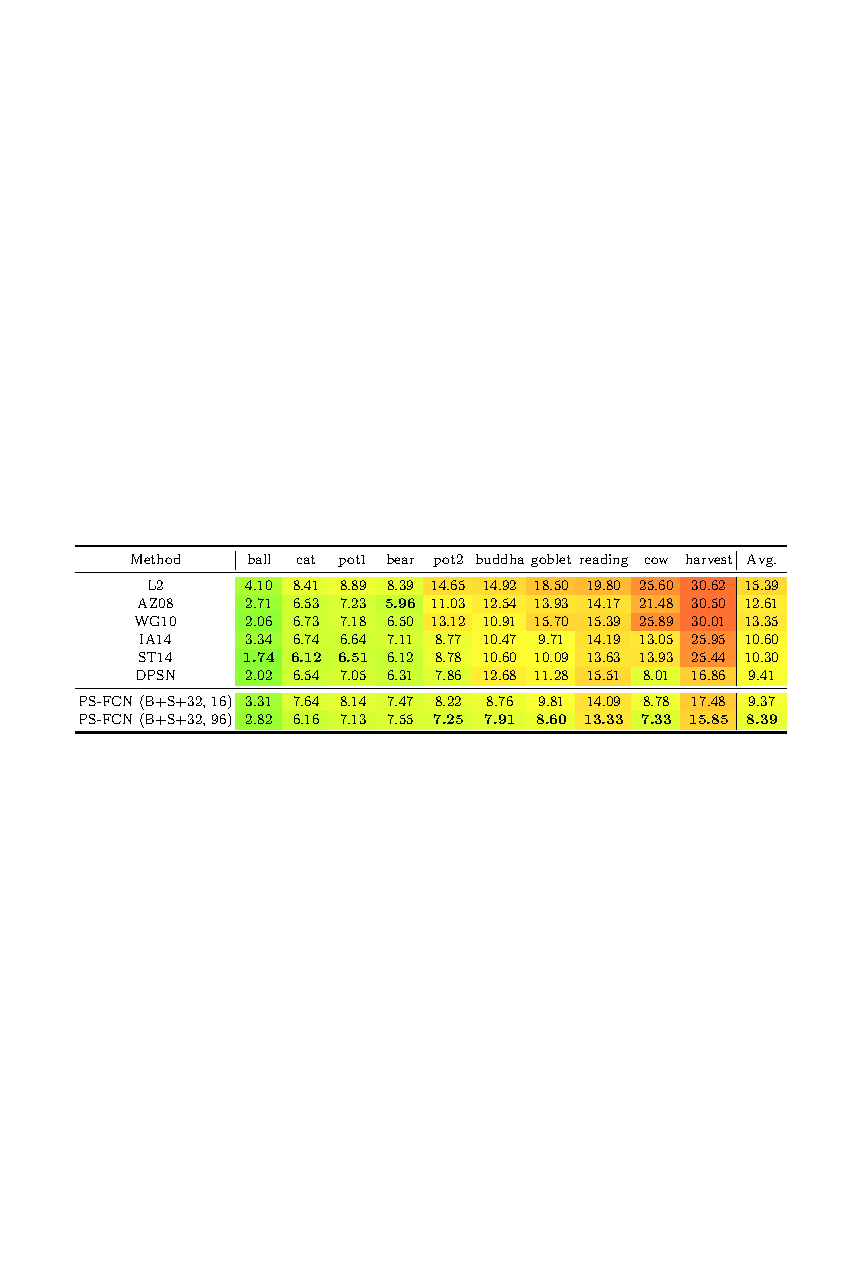
\includegraphics[width=0.98\textwidth]{images/res_quant_diligent_main}
        \end{center}
    \end{minipage}

    \vspace{0.5em}

    \begin{minipage}[t]{0.525\textwidth}
        \textbf{\color{sufered}Feature Visualization:}
        \vspace{-0.5em}
        \begin{center}
            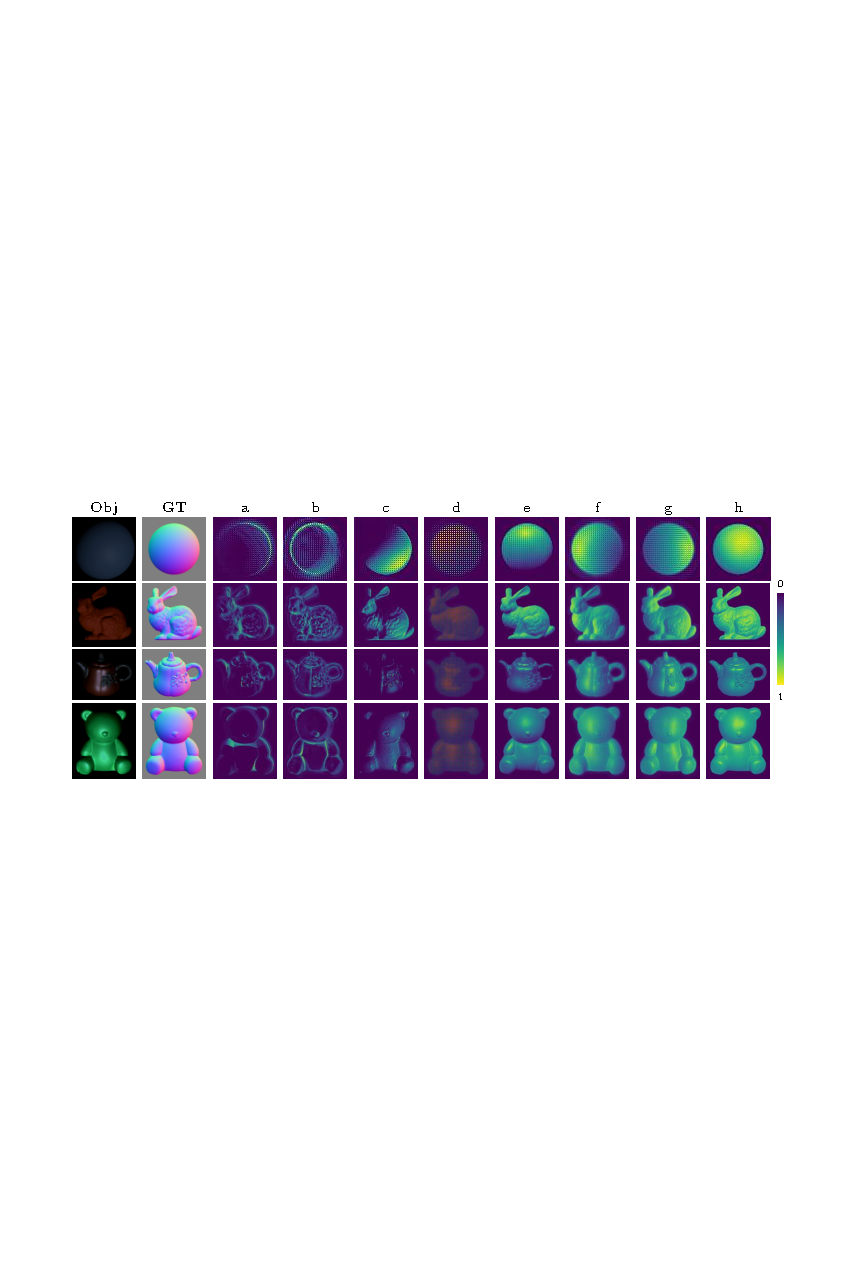
\includegraphics[width=\textwidth]{images/visualization}
        \end{center}
        \vspace{-0.9em}
        \begin{itemize}
            \item Different regions with similar normal directions are fired in different channels. Each channel can therefore be interpreted as the probability of the normal belonging to a certain direction.
        \end{itemize}
    \end{minipage}
    \hfill
    \begin{minipage}[t]{0.465\textwidth}
    \textbf{\color{sufered}Qualitative Results on DiLiGenT Main Dataset:} 
        \begin{center}
            \vspace{-0.5em}
            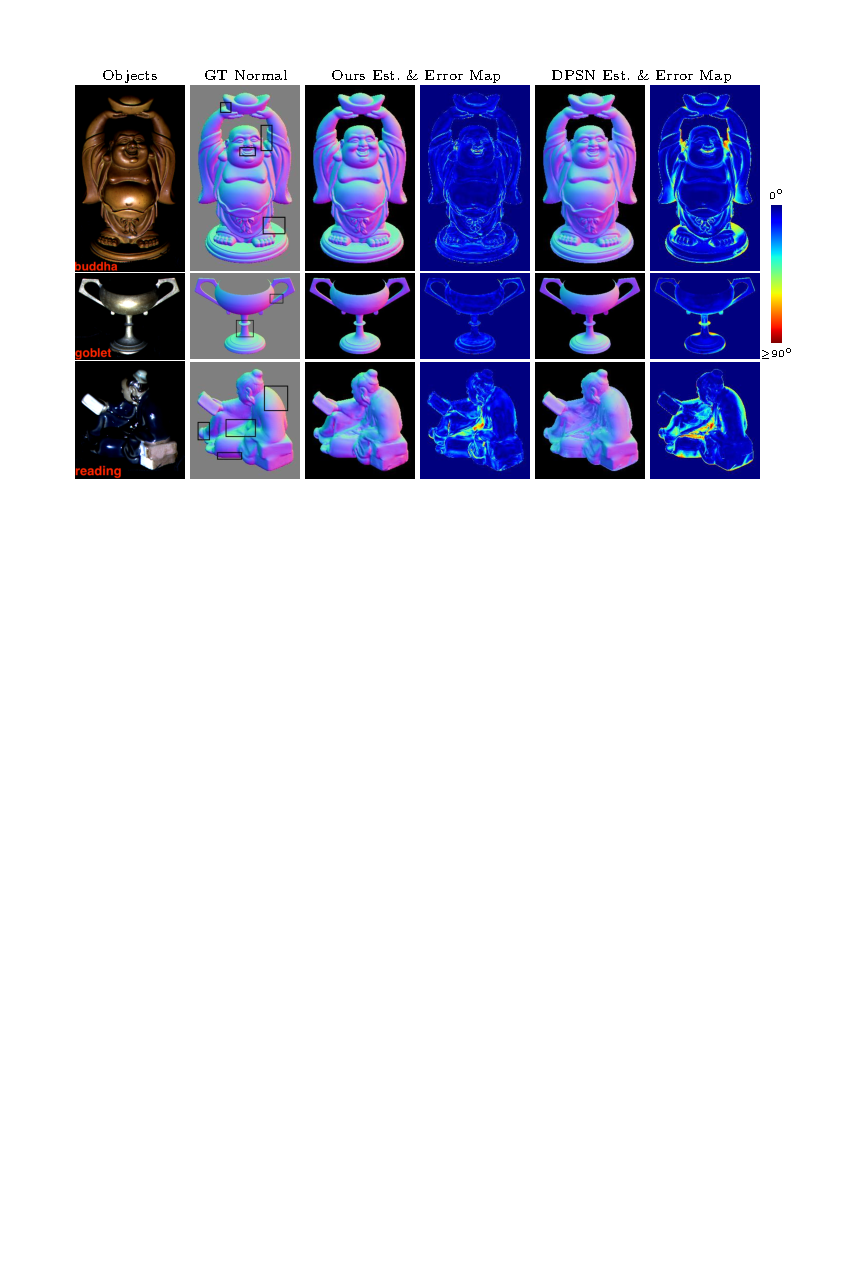
\includegraphics[width=\textwidth]{images/res_qual_diligent_main}
        \end{center}
    \end{minipage}

    \vspace{0.8em}
    \textbf{\color{sufered}Qualitative Results on the Gourd\&Apple Dataset and Light Stage Data Gallery:}
    \vspace{-0.8em}
    \begin{center}
        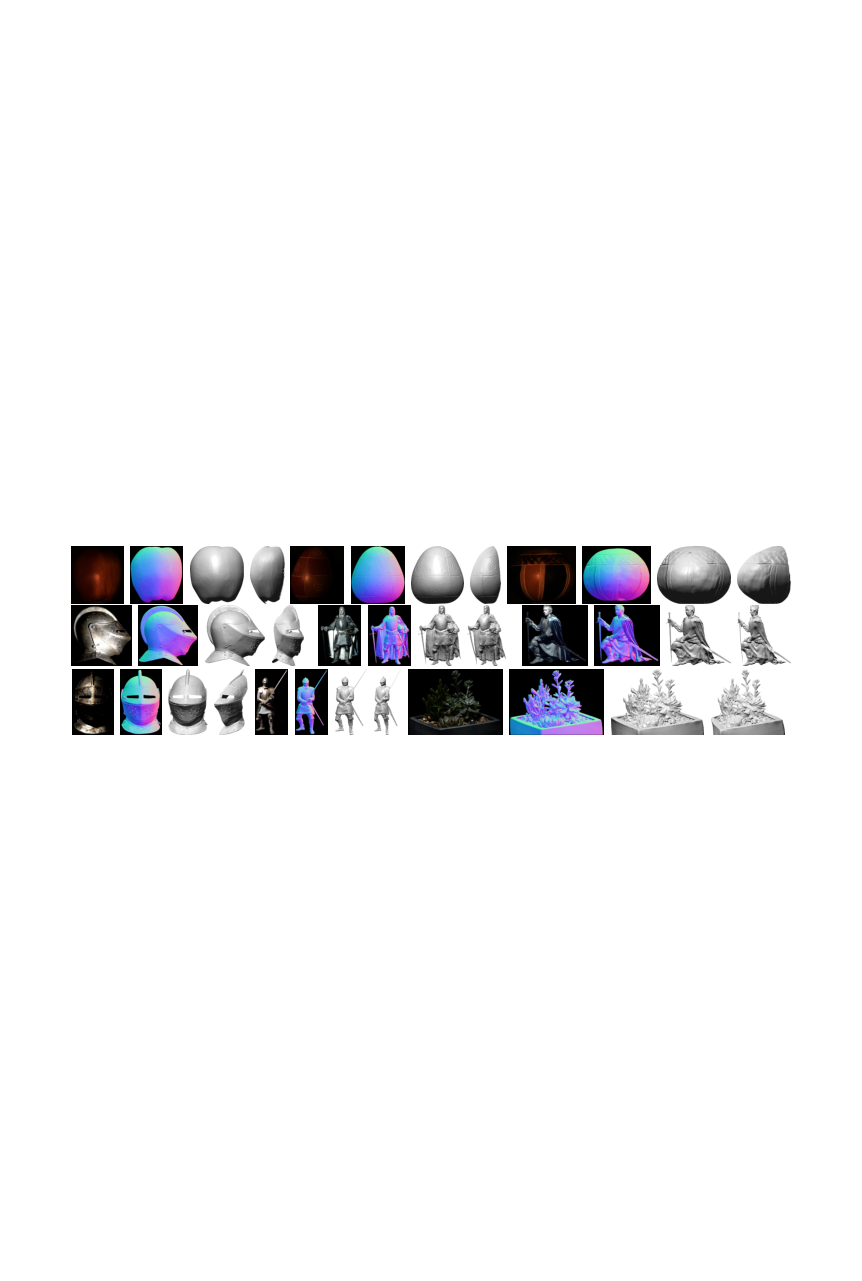
\includegraphics[width=1\textwidth]{images/gourd_stage}
    \end{center}

    \begin{minipage}[t]{0.6\textwidth}
        \textbf{\color{sufered}Quantitative Results on Spheres Rendered with 100 Different Materials:} 
        \vspace{-0.5em}
        \begin{center}
            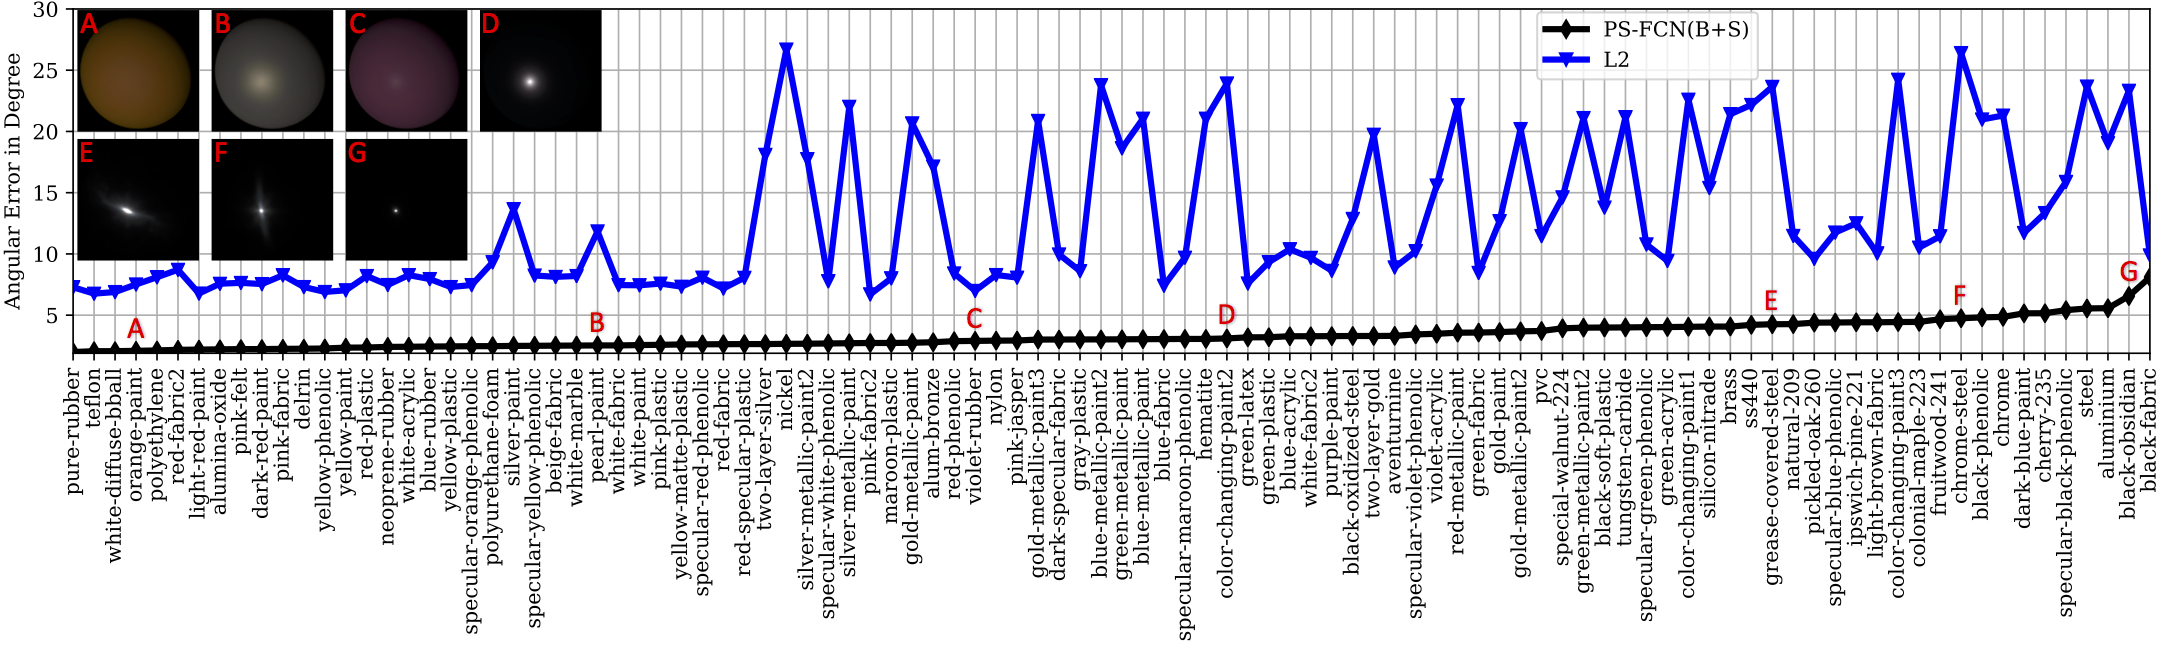
\includegraphics[width=\textwidth]{images/100brdf.png}
        \end{center}
    \end{minipage}
    \begin{minipage}[t]{0.4\textwidth}
        \textbf{\color{sufered}Quantitative Results of Uncalibrated PS-FCN on DiLiGenT Main Dataset:} 
        \vspace{-0.5em}
        \begin{center}
            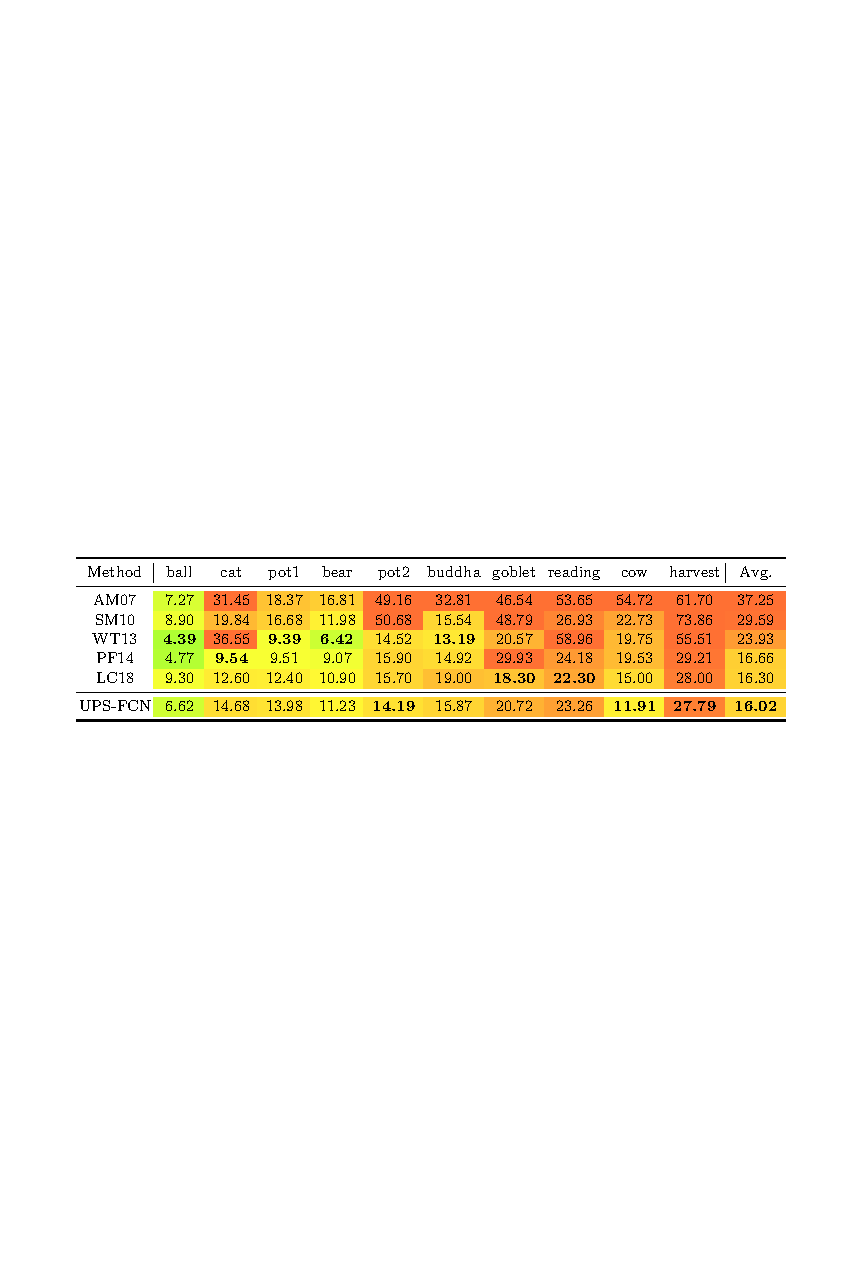
\includegraphics[width=\textwidth]{images/res_uncalibrated}
        \end{center}
        \vspace{-1.5em}

        \begin{center}
        \begin{minipage}{0.56\linewidth}
            \begin{center}
            \textbf{Project Webpage}: \\
            \vspace{0.5em}\textbf{Code} \& \textbf{Dataset} \& \textbf{Model}
            \end{center}
        \end{minipage}
        \begin{minipage}{0.24\linewidth}
            \begin{center}
                
\includegraphics[width=\linewidth]{images/PS-FCN_QRCode.png}
            \end{center}
        \end{minipage}
        \end{center}
    \end{minipage}
}

    \end{poster}
\end{document}